% Slide 29: The Data Mining Process
\begin{frame}{فرآیند کشف دانش در داده‌ها (\lr{KDD})}
\begin{itemize}
  \item \textbf{مدل کلاسیک فرآیند کشف دانش در پایگاه‌های داده} (\lr{Fayyad et al., 1996})
\end{itemize}
\begin{center}
  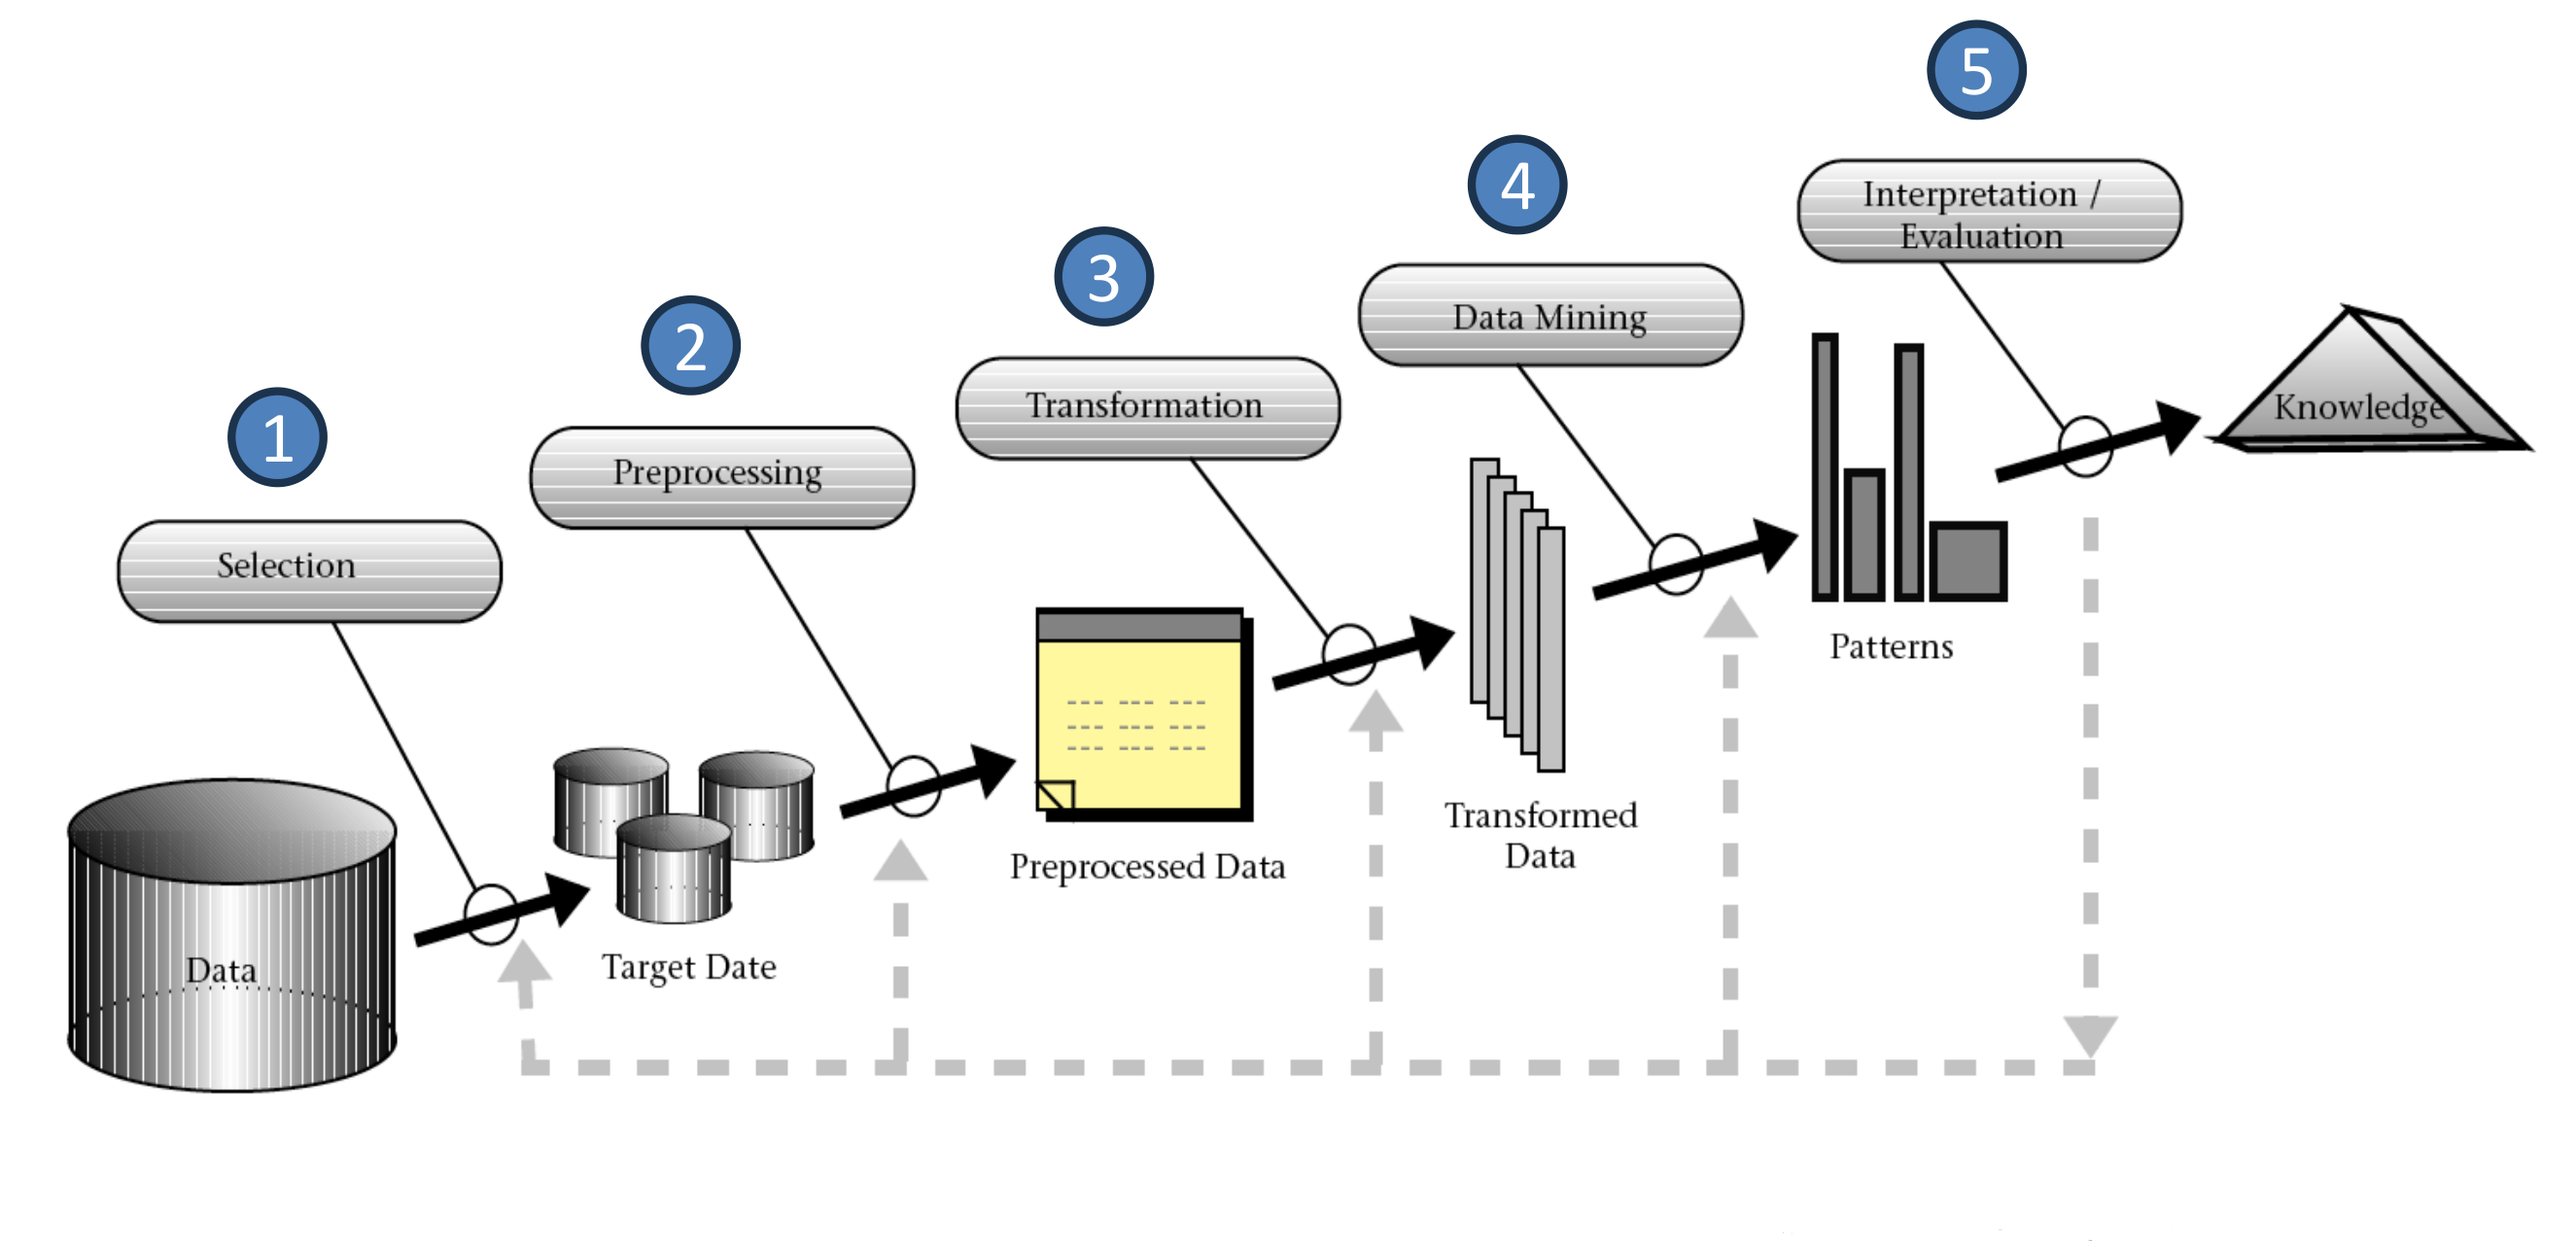
\includegraphics[width=0.92\textwidth,height=4cm,keepaspectratio]{images/img_p29_1_158.png}\\[0.15cm]
  {\fontsize{6.8}{8}\selectfont\color{subgray}پنج گام اصلی: انتخاب $\leftarrow$ پیش‌پردازش $\leftarrow$ تبدیل داده‌ها $\leftarrow$ داده‌کاوی $\leftarrow$ ارزیابی و تفسیر}
\end{center}
\end{frame}

% Slide 30: Selection and Exploration (1)
\begin{frame}{گام اول -- انتخاب و اکتشاف داده‌ها}
\framesubtitle{\lr{Selection and Exploration}}
\begin{columns}[T,onlytextwidth]
\begin{column}{0.62\textwidth}
\begin{itemize}
  \item \textbf{انتخاب داده‌ها (\lr{Selection})}
  \begin{itemize}
    \item چه داده‌هایی در دسترس داریم؟
    \item کدام بخش از داده‌ها برای مسئله مد نظر مفید و مرتبط هستند؟
    \item از کیفیت، پیشینه و اعتبار داده‌ها چه می‌دانیم؟
  \end{itemize}
  \vspace{0.2cm}
  \item \textbf{اکتشاف و پروفایل‌سازی (\lr{Exploration / Profiling})}
  \begin{itemize}
    \item کسب درک و شهود اولیه از ساختار مجموعه‌داده
    \item محاسبه آماره‌های توصیفی (میانگین، واریانس، چارک‌ها)
    \item مصورسازی و رسم نمودارهای توزیع ویژگی‌ها
    \item شناسایی داده‌های پرت (\lr{Outliers})، مقادیر گمشده و رکوردهای تکراری
  \end{itemize}
\end{itemize}
\end{column}
\begin{column}{0.35\textwidth}
\begin{center}
  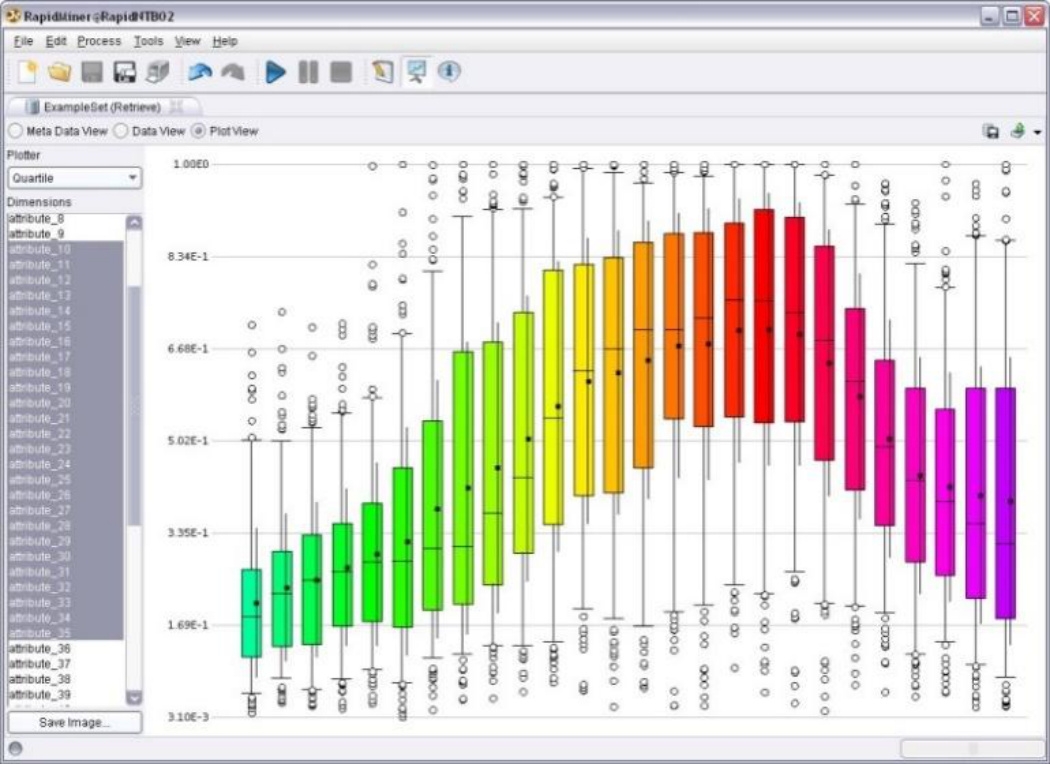
\includegraphics[width=\textwidth,height=2.2cm,keepaspectratio]{images/img_p30_1_161.jpeg}\\[0.2cm]
  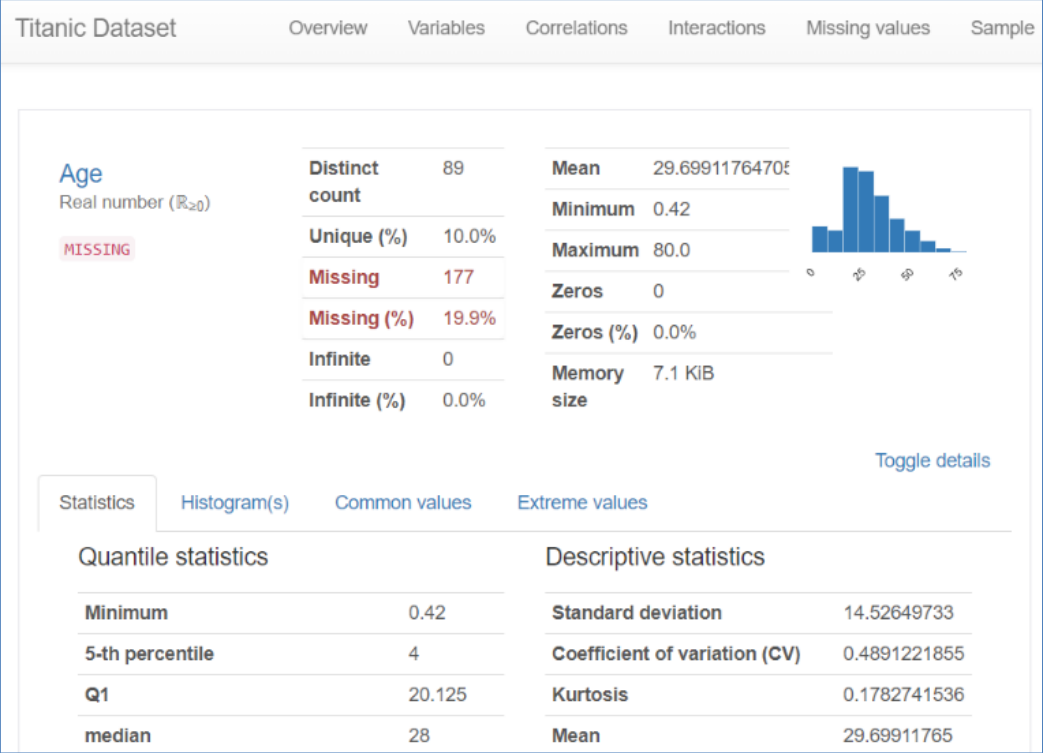
\includegraphics[width=\textwidth,height=2.2cm,keepaspectratio]{images/img_p30_2_162.png}
\end{center}
\end{column}
\end{columns}
\end{frame}

% Slide 31: Preprocessing and Transformation (2+3)
\begin{frame}{گام‌های دوم و سوم -- پیش‌پردازش و تبدیل داده‌ها}
\framesubtitle{\lr{Preprocessing and Transformation}}
\begin{columns}[T,onlytextwidth]
\begin{column}{0.65\textwidth}
\begin{itemize}
  \item \textbf{تبدیل به فرمت سازگار با الگوریتم‌های داده‌کاوی:}
  \begin{itemize}
    \item ابعاد ویژگی‌ها: بازنمایی داده با کمترین تعداد مشخصه مناسب
    \item مقیاس ویژگی‌ها: اسمی (\lr{Nominal})، ترتیبی (\lr{Ordinal})، عددی پیوسته
    \item حجم داده: هماهنگی با توان محاسباتی و حافظه
  \end{itemize}
  \vspace{0.2cm}
  \item \textbf{تکنیک‌های کلیدی مهندسی داده:}
  \begin{itemize}
    \item گسسته‌سازی و باینری‌کردن متغیرها
    \item انتخاب ویژگی (\lr{Feature Selection}) و کاهش ابعاد (\lr{PCA})
    \item تبدیل متن به بردارهای وزنی و تعبیه‌ها (\lr{Embeddings})
    \item تجمیع داده‌ها (\lr{Aggregation}) و نمونه‌برداری (\lr{Sampling})
    \item ادغام داده‌ها از منابع ناهمگون سازمانی
  \end{itemize}
\end{itemize}
\end{column}
\begin{column}{0.32\textwidth}
\begin{center}
  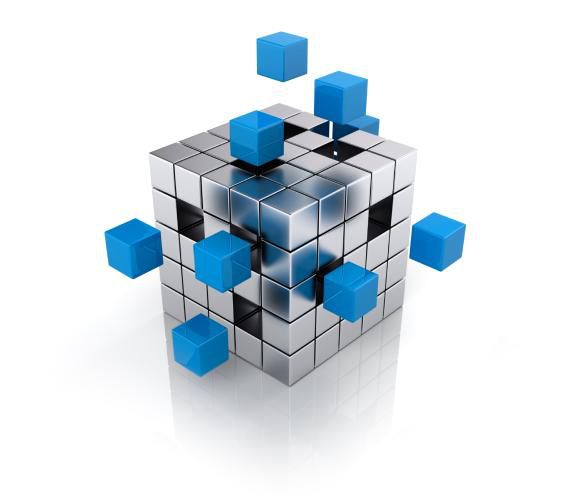
\includegraphics[width=\textwidth,height=4cm,keepaspectratio]{images/img_p31_1_165.jpeg}
\end{center}
\end{column}
\end{columns}
\end{frame}

% Slide 32: Preprocessing - Effort
\begin{frame}{اهمیت و زمان‌بری پیش‌پردازش داده‌ها}
\begin{itemize}
  \item \textbf{آماده‌سازی داده‌ها، کلید ساخت مدل‌های معتبر:}
  \begin{itemize}
    \item کیفیت مدل نهایی مستقیماً وابسته به کیفیت داده‌های ورودی است.
    \item طبق گزارش معتبر شرکت \lr{CrowdFlower}، پاک‌سازی و ادغام داده‌ها حدود \textbf{\lr{70\% -- 80\%}} از زمان و انرژی متخصصان را به خود اختصاص می‌دهد!
  \end{itemize}
  \vspace{0.15cm}
  \item \textbf{درس مرتبط در دانشگاه مانهایم:} \lr{IE670 Web Data Integration}
\end{itemize}
\begin{center}
  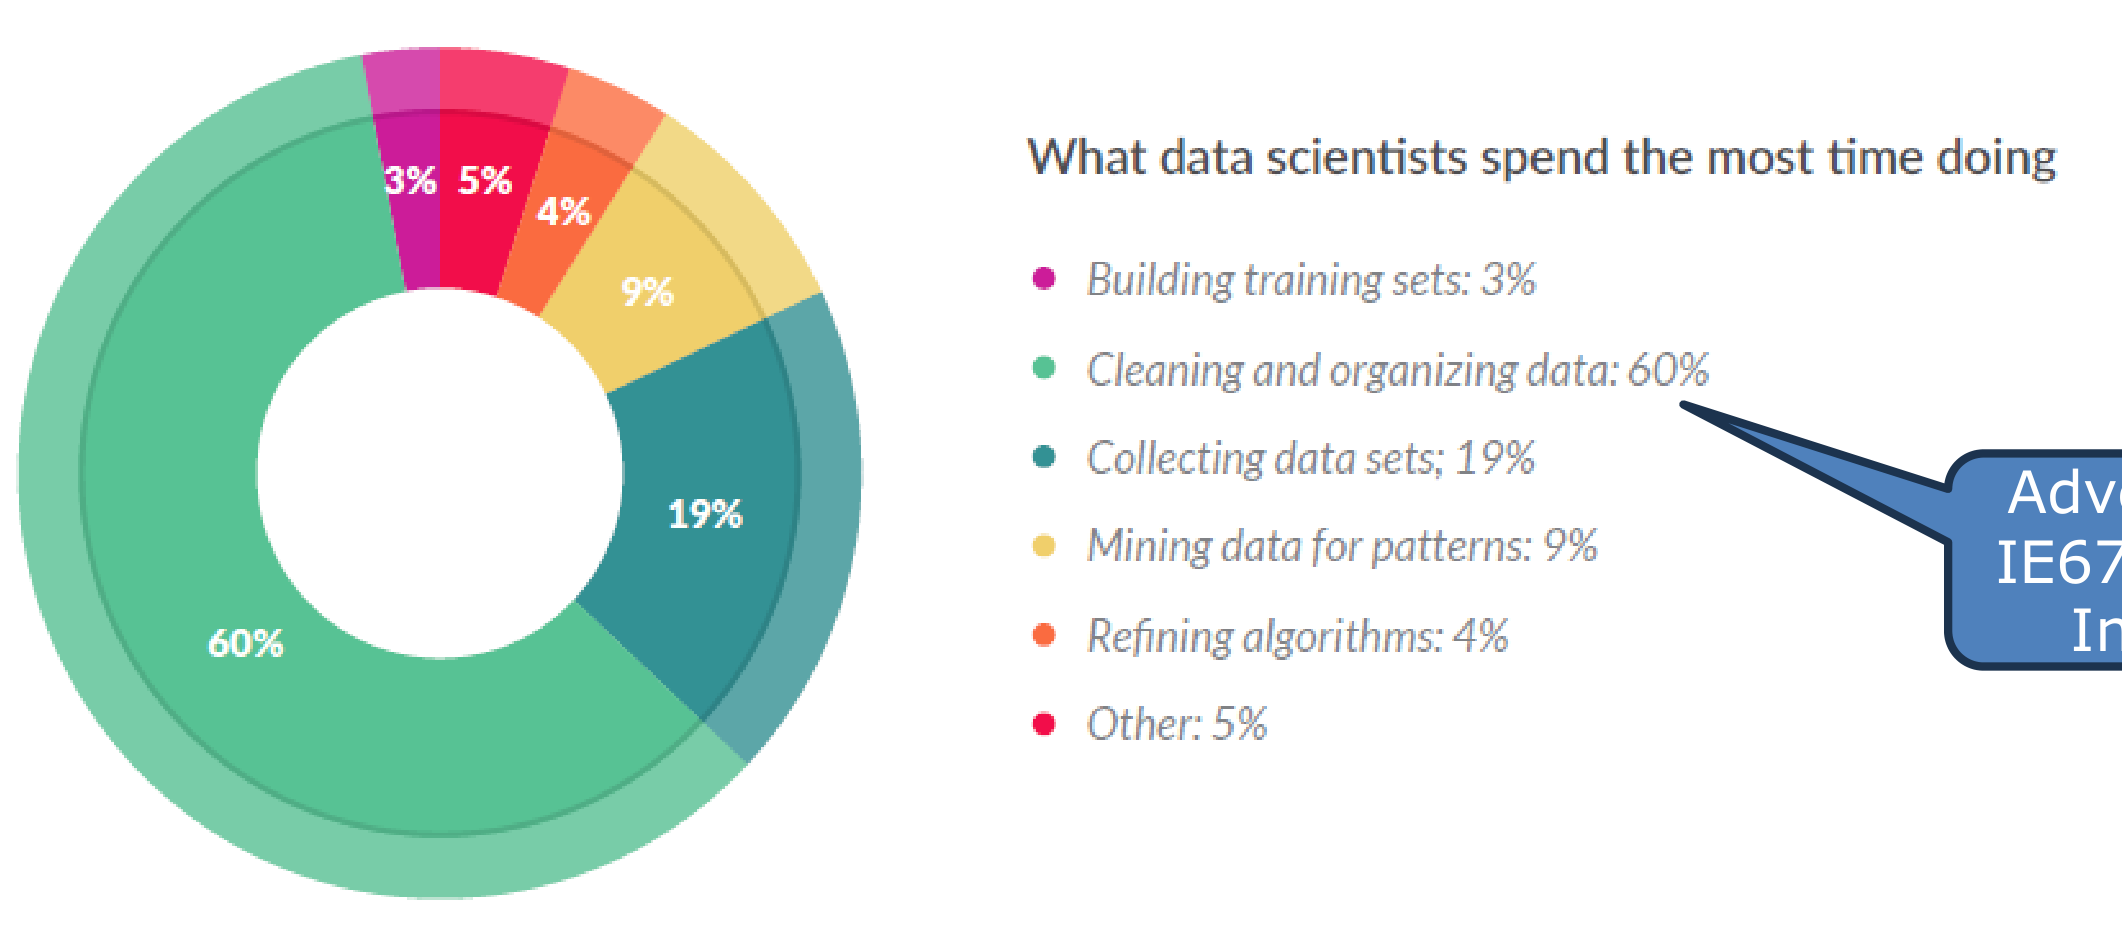
\includegraphics[width=0.72\textwidth,height=3.4cm,keepaspectratio]{images/img_p32_2_173.png}
\end{center}
\end{frame}

% Slide 33: Data Mining (4)
\begin{frame}{گام چهارم -- داده‌کاوی و یادگیری مدل}
\framesubtitle{\lr{Data Mining}}
\begin{columns}[T,onlytextwidth]
\begin{column}{0.65\textwidth}
\begin{itemize}
  \item \textbf{ورودی:} داده‌های پیش‌پردازش‌شده
  \item \textbf{خروجی:} الگوها و مدل‌های استخراج‌شده
  \vspace{0.2cm}
  \item \textbf{فرآیند تکرارشونده و چرخه‌ای:}
  \begin{enumerate}
    \item اعمال الگوریتم داده‌کاوی روی داده‌ها
    \item ارزیابی عملکرد و کارایی مدل یا الگوها
    \item اصلاح و تکرار چرخه:
    \begin{itemize}
      \item آزمایش با هایپرپارامترهای مختلف
      \item امتحان روش‌ها و الگوریتم‌های جایگزین
      \item بازنگری در پیش‌پردازش و مهندسی ویژگی‌ها
      \item افزایش کمیت و کیفیت داده‌های آموزش
      \item ترکیب نتایج مدل‌های مختلف (\lr{Ensemble})
    \end{itemize}
  \end{enumerate}
\end{itemize}
\end{column}
\begin{column}{0.32\textwidth}
\begin{center}
  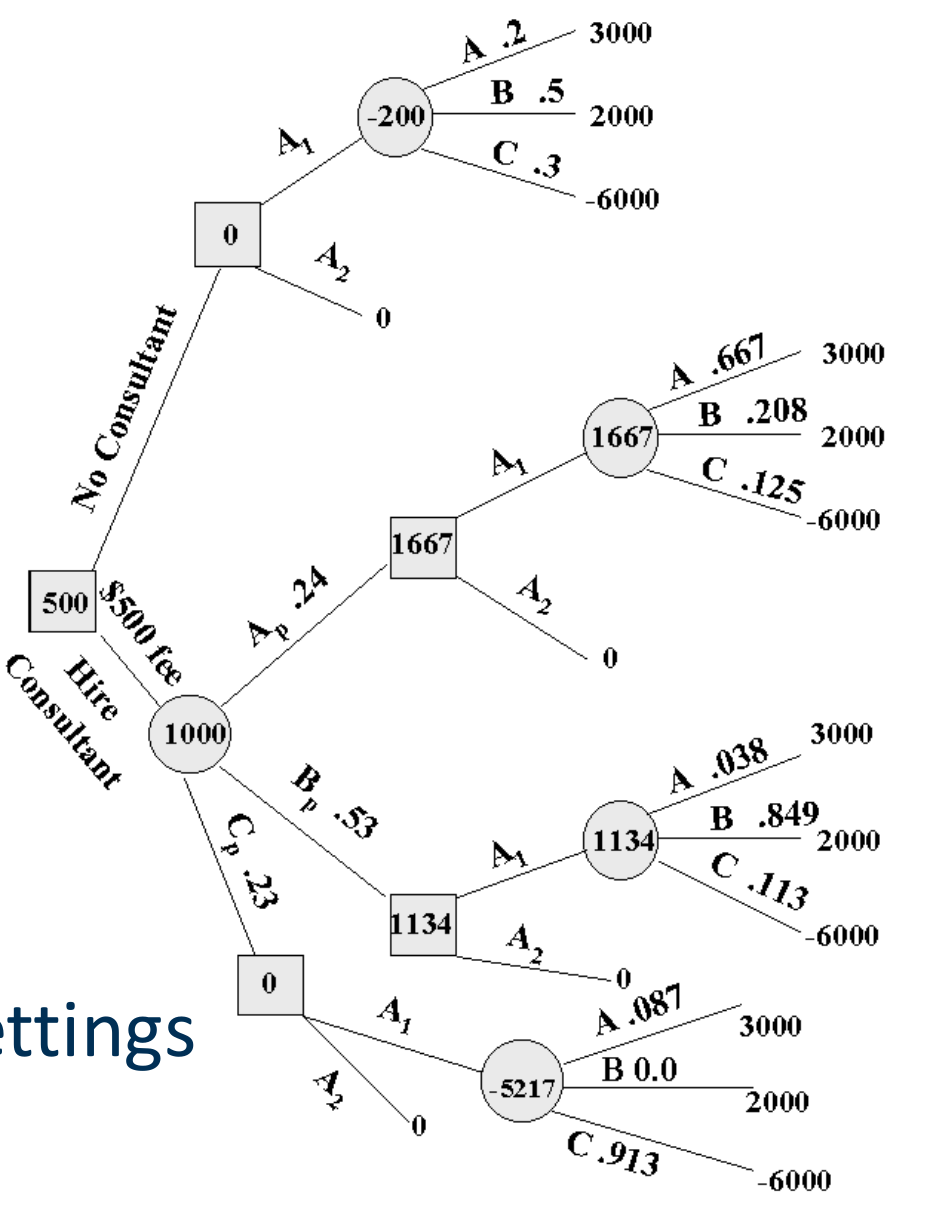
\includegraphics[width=\textwidth,height=4.2cm,keepaspectratio]{images/img_p33_1_176.png}
\end{center}
\end{column}
\end{columns}
\end{frame}

% Slide 34: Interpretation / Evaluation (5)
\begin{frame}{گام پنجم -- تفسیر، ارزیابی و ارزش‌آفرینی}
\framesubtitle{\lr{Interpretation / Evaluation}}
\begin{columns}[T,onlytextwidth]
\begin{column}{0.65\textwidth}
\begin{itemize}
  \item \textbf{خروجی فرآیند داده‌کاوی:}
  \begin{itemize}
    \item الگوهای کشف‌شده (\lr{Patterns})
    \item مدل‌های آماری و ریاضیاتی (\lr{Models})
  \end{itemize}
  \vspace{0.3cm}
  \item \textbf{هدف غایی: خلق ارزش واقعی برای سازمان:}
  \begin{itemize}
    \item کسب بینش عمیق و دانش عملیاتی (\lr{Gain Knowledge})
    \item اتخاذ تصمیم‌های آگاهانه‌تر و بهینه (\lr{Better Decisions})
    \item افزایش درآمد و کاهش هزینه‌ها (\lr{Increase Revenue})
  \end{itemize}
\end{itemize}
\end{column}
\begin{column}{0.32\textwidth}
\begin{center}
  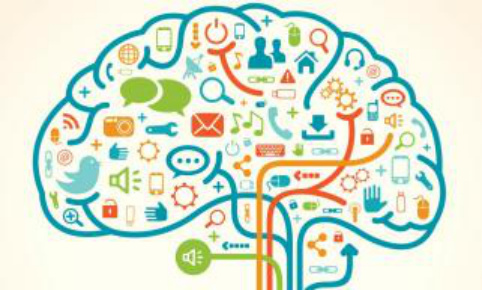
\includegraphics[width=0.85\textwidth,height=1.2cm,keepaspectratio]{images/img_p34_2_180.jpeg}\\[0.1cm]
  
\includegraphics[width=0.85\textwidth,height=1.2cm,keepaspectratio]{images/img_p34_3_181.jpeg}\\[0.1cm]
  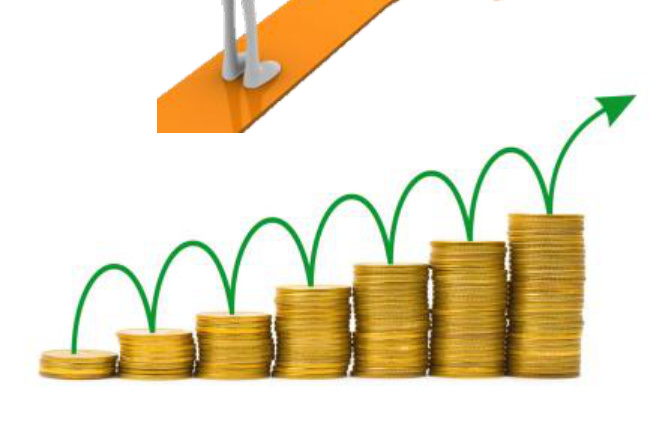
\includegraphics[width=0.85\textwidth,height=1.2cm,keepaspectratio]{images/img_p34_1_179.jpeg}
\end{center}
\end{column}
\end{columns}
\end{frame}

% Slide 35: Deployment (CRISP-DM)
\begin{frame}{استقرار مدل و چرخه فرآیندی \lr{CRISP-DM}}
\framesubtitle{\lr{Deployment \& CRISP-DM Process Model}}
\begin{itemize}
  \item \textbf{به‌کارگیری عملیاتی مدل در بستر سیستم‌ها و فرآیندهای کسب‌وکار}
  \item \textbf{تکرار مداوم چرخه به منظور پایش، نگهداری و بهبود مستمر عملکرد مدل}
\end{itemize}
\begin{center}
  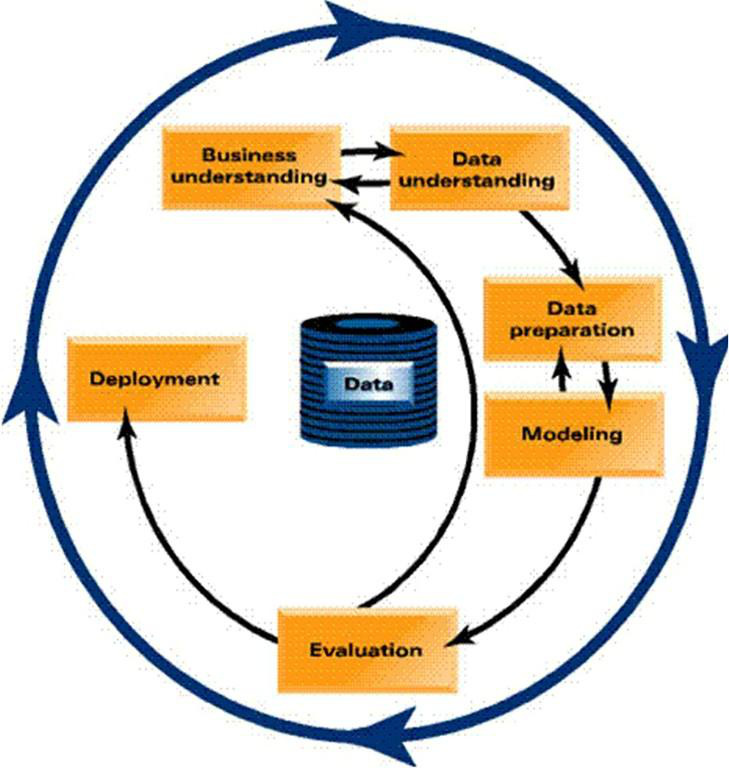
\includegraphics[height=3.5cm,keepaspectratio]{images/img_p35_1_185.jpeg}\\[0.15cm]
  {\small\textbf{مدل فرآیندی استاندارد کریسپ (\lr{CRISP-DM Process Model})}}
\end{center}
\end{frame}
